\documentclass{tufte-handout}\usepackage[]{graphicx}\usepackage[]{color}
%% maxwidth is the original width if it is less than linewidth
%% otherwise use linewidth (to make sure the graphics do not exceed the margin)
\makeatletter
\def\maxwidth{ %
  \ifdim\Gin@nat@width>\linewidth
    \linewidth
  \else
    \Gin@nat@width
  \fi
}
\makeatother

\definecolor{fgcolor}{rgb}{0.345, 0.345, 0.345}
\newcommand{\hlnum}[1]{\textcolor[rgb]{0.686,0.059,0.569}{#1}}%
\newcommand{\hlstr}[1]{\textcolor[rgb]{0.192,0.494,0.8}{#1}}%
\newcommand{\hlcom}[1]{\textcolor[rgb]{0.678,0.584,0.686}{\textit{#1}}}%
\newcommand{\hlopt}[1]{\textcolor[rgb]{0,0,0}{#1}}%
\newcommand{\hlstd}[1]{\textcolor[rgb]{0.345,0.345,0.345}{#1}}%
\newcommand{\hlkwa}[1]{\textcolor[rgb]{0.161,0.373,0.58}{\textbf{#1}}}%
\newcommand{\hlkwb}[1]{\textcolor[rgb]{0.69,0.353,0.396}{#1}}%
\newcommand{\hlkwc}[1]{\textcolor[rgb]{0.333,0.667,0.333}{#1}}%
\newcommand{\hlkwd}[1]{\textcolor[rgb]{0.737,0.353,0.396}{\textbf{#1}}}%
\let\hlipl\hlkwb

\usepackage{framed}
\makeatletter
\newenvironment{kframe}{%
 \def\at@end@of@kframe{}%
 \ifinner\ifhmode%
  \def\at@end@of@kframe{\end{minipage}}%
  \begin{minipage}{\columnwidth}%
 \fi\fi%
 \def\FrameCommand##1{\hskip\@totalleftmargin \hskip-\fboxsep
 \colorbox{shadecolor}{##1}\hskip-\fboxsep
     % There is no \\@totalrightmargin, so:
     \hskip-\linewidth \hskip-\@totalleftmargin \hskip\columnwidth}%
 \MakeFramed {\advance\hsize-\width
   \@totalleftmargin\z@ \linewidth\hsize
   \@setminipage}}%
 {\par\unskip\endMakeFramed%
 \at@end@of@kframe}
\makeatother

\definecolor{shadecolor}{rgb}{.97, .97, .97}
\definecolor{messagecolor}{rgb}{0, 0, 0}
\definecolor{warningcolor}{rgb}{1, 0, 1}
\definecolor{errorcolor}{rgb}{1, 0, 0}
\newenvironment{knitrout}{}{} % an empty environment to be redefined in TeX

\usepackage{alltt}

%\geometry{showframe}% for debugging purposes -- displays the margins
\usepackage{verbatim}
\usepackage{amsmath}
\usepackage{hyperref}
%\usepackage{natbib}
%\bibfont{\small} % Doesn't see to work...

% Set up the images/graphics package
\usepackage{graphicx}
%\setkeys{Gin}{width=\linewidth,totalheight=\textheight,keepaspectratio}
% \graphicspath{{graphics/}}

\title{Confidence Interval Tutorial Assignment %\thanks{}
}
\author[Marc Los Huertos]{Marc Los Huertos}
%\date{}  % if the \date{} command is left out, the current date will be used


% \SweaveOpts{prefix.string=graphics/plot} % Created a "graphics" subdirectory to 

\setsidenotefont{\color{blue}}
% \setcaptionfont{hfont commandsi}
% \setmarginnotefont{\color{blue}}
% \setcitationfont{\color{gray}}

% The following package makes prettier tables.  We're all about the bling!
%\usepackage{booktabs}

% Small sections of multiple columns
%\usepackage{multicol}

% These commands are used to pretty-print LaTeX commands
% command name -- adds backslash automatically
%\newcommand{\docpkg}[1]{\texttt{#1}}% package name
%\newcommand{\doccls}[1]{\texttt{#1}}% document class name
%\newcommand{\docclsopt}[1]{\texttt{#1}}% document class option name
\IfFileExists{upquote.sty}{\usepackage{upquote}}{}
\begin{document}
%\SweaveOpts{concordance=TRUE}

\maketitle% this prints the handout title, author, and date
\begin{abstract}
\noindent One of the most important considerations with univariate data are the development of confidence intervals. As you can probably guess, confidence intervals are based on the distribution of the data. There are two main approaches in developing confidence intervals. One relies on the use of theoretical probability distributions but there are a number of methods that do not rely on theoretical distributions. We will learn several methods because each are used in environmental sciences to varying degrees.
\end{abstract}

%\printclassoptions

% Setting up the margins, etc for R


\section{Assignment}

To create a guide for your peers about what are confidence intervals and how to create them using a univarite dataset (one set of numbers). 

Using R-studio, write up an short description and demonstration of how to do a confidence interval for the sample mean. 

\subsection{Rationale}

Learning statistics is challenging and teaching it even more so. But I'm convinced that we learn better if we are asked to teach a topic. 

\begin{marginfigure}
	\centering
		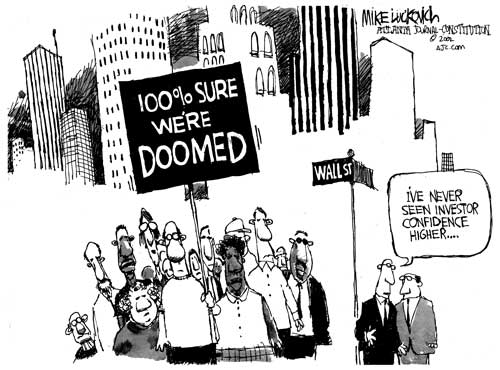
\includegraphics[width=1.00\textwidth]{Investor_confidence500.jpg}
	\caption{Confidence abounds without limits.}
	\label{fig:Investor_confidence500}
\end{marginfigure}

\subsection{Resources}

There are tons of resources to complete this assigment. For example, I have several statistics textbooks that might help you figure out how to talk about confidence intervals. 
There are numerous cheatsheets avaialble, which you can get from Rstudio (\texttt{Help/Cheetsheets}) or from Sakai (\texttt{Resources/Project 0 General Resources/Software Resources}). You might look at my \href{https://github.com/marclos/beginnersluck/raw/master/Confidence_Intervals/Confidence_Intervals.pdf}{Guidelines to Confidence Intervals} which is also linked to the Sakai page.\sidenote{I started this guide a few days ago and it's still pretty rough, but has many of the pieces you might need!}

I also suggest some good videos, e.g. Khan Academy, etc.:

\begin{itemize}
  \item \href{https://www.khanacademy.org/math/ap-statistics/estimating-confidence-ap/introduction-confidence-intervals/v/confidence-intervals-and-margin-of-error}{Confidence intervals for proprotions (Kahn Academy)}.
  \item \href{https://www.youtube.com/watch?v=tFWsuO9f74o}{Understanding Confidence Intervals: Statistics Help}
\end{itemize}


Finally, there are some good (and some terrible -- Read: Wrong) resources on the web as well. 

\subsection{Assignment Steps}

\begin{enumerate}
  \item (1 pnt) Successfully use R-studio to create a pdf from markdown;\sidenote{To open a markdown file, go to `File/New File/R Markdown'. This will open a template for you to modify.}
  \item (1 pnt) Create a title, e.g. ``Guide on Confidence Intervals for the Perplexed", or ``What is a Confidence Interval.'' You can changes these later if you want. Use your random number for the author name. Then select pdf to make sure your output is a pdf. You can changes these later so don't worry if you don't like your title or some other choice.
  \item (1 pnt) Replace the template text with a description of what is a confidence interval and how it depends on probability distributions; 
  \item (1 pnt) Describe ``how'' we talk about confidence intervals, relative to the population and sample means;
  \item (1 pnt) Generate a vector of 5 random numbers with a mean of 10 and standard deviation of 1;\sidenote{You should use \texttt{rnorm()} to accomplish this.}
  \item (1 pnt) Report the sample mean and standard deviation;
  \item (2 pnts) Calculate the confidence intervals for 95\% and 90\% and how we should report the results correctly in each case.
  \item (2 pnts) Create a probability distribution that shows the confidence intervals. This is the hardest part and relies on create a probability density curve. \sidenote{In my example this requires the use of \texttt{dnorm()}), where you'll need to create a dummy set of x values that encompose most of the potential x's in a sample and plot that relative to the height of the probability, calculated by\texttt{ dnorm()}.}. 
  
\end{enumerate}

Finally, I will also grade your guide based on the clarity and robustness of your approach (2 pnts). 

\section{Working an Example}

You can see that I have created a working example for myself, which you might find helpful or completely not!

here's the link for my \href{https://github.com/marclos/beginnersluck/raw/master/Confidence_Intervals/Confidence_Intervals.pdf}{Confidence Interval Guidelines}. 

As you work through your guide and find problems with mine, please point them out and I'll fix them!

\FloatBarrier 
\begin{fullwidth}
% \renewcommand{\bibfont}{\small}
%\bibliography{LosHuertos_Complete_100420}
%\bibliographystyle{cbe}
\end{fullwidth}

\end{document}
